\let\lesson\undefined
\newcommand{\lesson}{\phantomlesson{Bài 13: Tổng hợp lực song song cùng chiều}}
\chapter[Tổng hợp hai lực song song cùng chiều]{Tổng hợp hai lực song song cùng chiều}
\setcounter{section}{0}
\section{Lý thuyết}
Lực tổng hợp của hai lực song song cùng chiều là một lực:
\begin{itemize}
	\item Song song, cùng chiều với các lực thành phần.
	\item Có độ lớn bằng tổng độ lớn của các lực thành phần:
	$$F_t=F_1+F_2$$
	\item Có giá nằm trong mặt phẳng của hai lực thành phần, chia khoảng cách giữa hai giá của hai lực song song thành những đoạn tỉ lệ nghịch với độ lớn của hai lực ấy
	$$\dfrac{F_1}{F_2}=\dfrac{d_2}{d_1}.$$
\end{itemize}
\begin{center}
	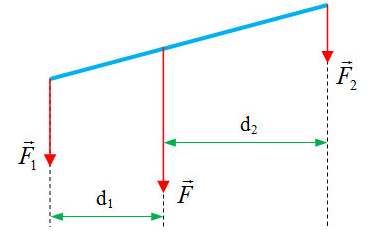
\includegraphics[width=0.35\linewidth]{../figs/VN10-2023-PH-TP022-2}
\end{center}
\section{Mục tiêu bài học - Ví dụ minh hoạ}
\begin{dang}{Xác định lực tổng hợp của hai lực song song cùng chiều}
	\viduii{3}
	{Một người đang gánh lúa như hình \ref{fig:22.2}. Hỏi vai người phải đặt ở vị trí nào trên đòn gánh để đòn gánh có thể nằm ngang cân bằng trong quá trình di chuyển? Biết khối lượng hai bó lúa lần lượt là $m_1=\SI{7}{\kilogram}$, $m_2=\SI{5}{\kilogram}$ và chiều dài đòn gánh là $\SI{1.5}{\meter}$. Xem như điểm treo hai bó lúa sát hai đầu đòn gánh và bỏ qua khối lượng đòn gánh.
	\begin{center}
		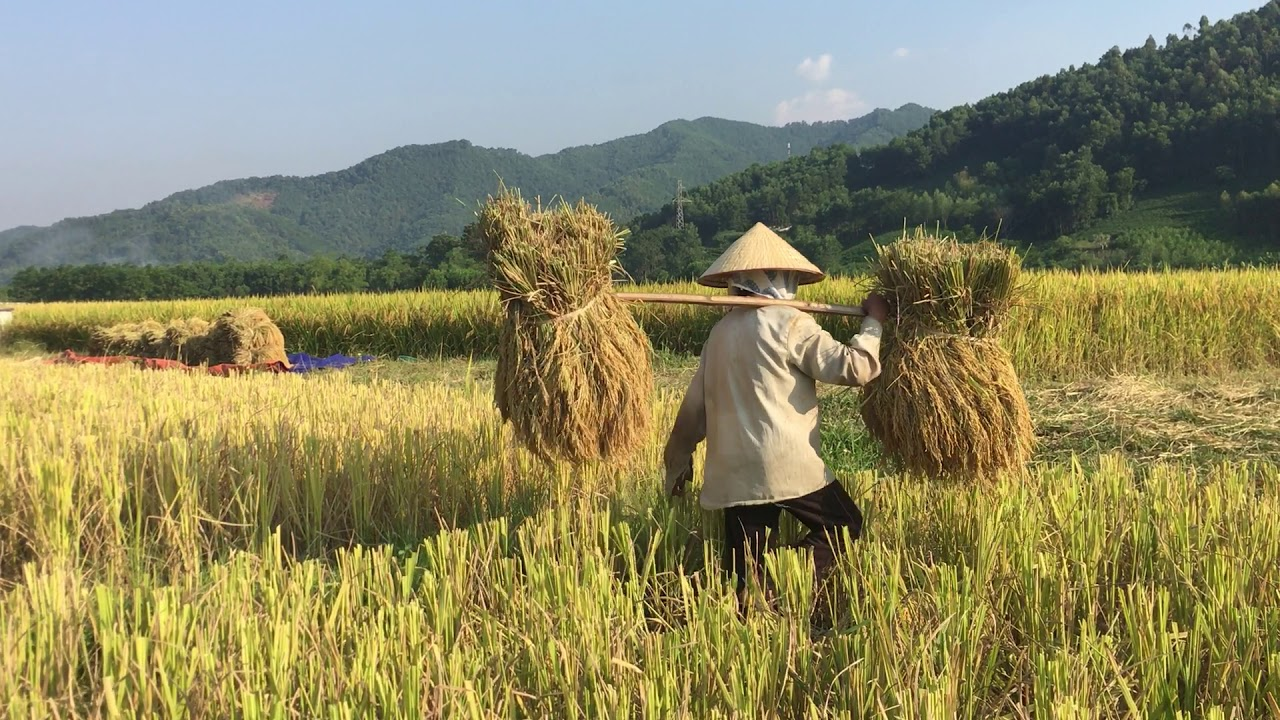
\includegraphics[width=0.3\linewidth]{../figs/VN10-2023-PH-TP022-1}
		\captionof{figure}{Người nông dân gánh lúa ở hai đầu đòn gánh.}
		\label{fig:22.2}
	\end{center}
}
{\begin{center}
		\textbf{Hướng dẫn giải}
	\end{center}
Áp dụng quy tắc tổng hợp lực song song cùng chiều, để đòn gánh cân bằng thì
\begin{equation}
	\label{eq:22.1}
	\dfrac{d_2}{d_1}=\dfrac{F_1}{F_2}=\dfrac{m_1g}{m_2g}=\dfrac{7}{5}
\end{equation}
mà
\begin{equation}
	\label{eq:22.2}
	d_1+d_2=\SI{1.5}{\meter}
\end{equation}
Từ (\ref{eq:22.1}) và (\ref{eq:22.2}), ta thu được:
\begin{align*}
	\begin{cases}
		d_1=\SI{0.625}{\meter}\\
		d_2=\SI{0.875}{\meter}.
	\end{cases}
\end{align*}
}
	\viduii{3}
	{Hai người khiêng một thùng hàng khối lượng $\SI{30}{\kilogram}$ bằng một đòn tre dài $\SI{2}{\meter}$ như hình \ref{fig:22.3}. Hỏi phải treo thùng hàng ở điểm nào để lực đè lên vai người đi sau lớn hơn lực đè lên vai người đi trước $\SI{100}{\newton}$. Bỏ qua khối lượng của đòn tre. Lấy $g=\SI{10}{\meter/\second^2}$.
		\begin{center}
			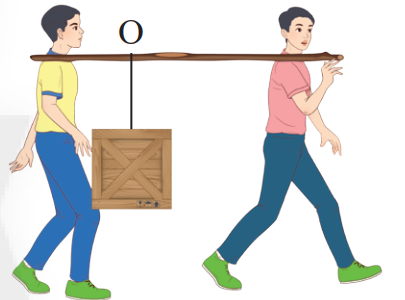
\includegraphics[width=0.3\linewidth]{../figs/VN10-2023-PH-TP022-3}
			\captionof{figure}{Hai bạn khiêng thùng hàng.}
			\label{fig:22.3}
		\end{center}
	}
	{\begin{center}
			\textbf{Hướng dẫn giải}
		\end{center}
		Gọi $F_1$, $F_2$ lần lượt là lực do đòn gánh đè lên vai người đi trước và người đi sau.\\
		Lực đè lên vai người đi sau lớn hơn lực đè lên vai người đi trước $\SI{100}{\newton}$:
		\begin{equation}
			\label{eq:22.3}
			F_2-F_1=\SI{100}{\newton}
		\end{equation}
		Tổng hợp lực đè lên vai 2 người bằng trọng lực của thùng hàng:
		\begin{equation}
			\label{eq:22.4}
			F_1+F_2=mg=\SI{300}{\newton}
		\end{equation}
		Từ (\ref{eq:22.3}) và (\ref{eq:22.4}), thu được:
		$$F_1=\SI{100}{\newton}; \quad F_2=\SI{200}{\newton}$$
		Áp dụng quy tắc tổng hợp lực song song cùng chiều:
		\begin{equation}
			\label{eq:22.5}
			\dfrac{d_2}{d_1}=\dfrac{F_1}{F_2}=\dfrac{1}{2}
		\end{equation}
		Mặt khác:
		\begin{equation}
			\label{eq:22.6}
			d_1+d_2=\SI{2}{\meter}
		\end{equation}
		Từ (\ref{eq:22.5}) và (\ref{eq:22.6}), suy ra được:
		$$d_1=\xsi{\dfrac{4}{3}}{\meter}\approx\SI{1.33}{\meter}; \quad d_2=\xsi{\dfrac{2}{3}}{\meter}\approx\SI{0.67}{\meter}.$$
	}
\end{dang}